\subsection{Pipes and Filters}
Die höchste Abstraktion stellt das \first{Pipes and
Filters}-Patten dar:
\index{Architekturmuster!Pipes and Filters}

\begin{figure}[htbp]
	\begin{center}
		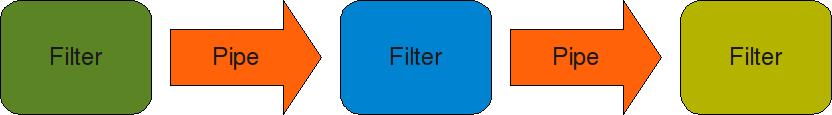
\includegraphics[scale=0.7]{pics/pipesFilter3.png}
	\caption[Pipes and Filter]{
	\textbf{Das Pipes and Filter Pattern}
	ist ein Architekturmuster für Systeme, um einen Strom von Daten zu
	verarbeiten.
	Jeder Verarbeitungsschritt ist in einen eigenen Filterkomponenten gekapselt.
	Die Daten werden dabei durch \name{Pipes} geleitet, die benachbarte
	\name{Filter} verbinden.
	Durch die Kapselung der Filter können diese rekombiniert werden, umso Familien
	von verwandten Systemem zu erstellen.
	\citep{buschmann_pattern-oriented_1996}}
	\end{center}
	\label{fig:pipesFilter}
\end{figure}

Die zu annotierende Sequenz wird schrittweise durch verschiedene \first{Filter}
bearbeitet. Jeder Filter, der in der \first{Pipeline} vorhanden ist, wird dabei
das entgültige Ergebnis der Annotation durch seine spezifischen Ergebnisse
erweitern.

Der Input eines Filters besteht dabei zum einen aus der zu
annotierenden Sequenz selbst, zum anderen aus einem zentralen Datenobjekt, in
dem alle gewonnenen Ergebnisse abgespeichert werden.
Ein Filter kann dabei auch auf die Ergebnisse eines anderen
Filters zugreifen oder auch angewiesen sein.
Die Reihenfolge der Filter innerhalb der Pipeline wird
somit durch die spezifischen \first{execution preconditions}
\footnote{\todo{execution precondition}}
aller Filter festgelegt.
\index{Filter}
\index{execution precondition}

Es ist davon auszugehen, dass die Ausführung einzelner Filter mitunter sehr
zeitintensiv sein wird. Ausserdem soll Nutzen aus dem im Institut installierten
\first{LSF} gezogen werden. Daher wird eine rein sequenzielle Abfolge der
Filter, wie es das Entwursmuster suggeriert, vermieden werden.
Stattdessen kann die Ausführung einzelner Filter parallel erfolgen.
Sind zu einem Zeitpunkt die execution preconditions mehrerer Filter erfüllt,
werden diese sofort zur Ausführung gebracht.
\index{Platform LSF}

Die Pipeline soll möglichst leicht konfigurierbar sein und sich an
individuelle Bedürfnisse anpassen lassen.
Vor diesem Hintergrund soll die Pipeline die veränderbaren Steps und das
statische \enquote{Ausführungsgerüst} vollständig entkoppeln. Beim Starten der
Pipeline soll diese an einem bestimmten Ort (lokales Verzeichnis oder
entferntes Repository) nach vorhandenen Steps suchen und diese in der Pipeline
installieren.

Die \name{Filter} des \name{pipes and filters} pattern sind somit aus der
eigentlichen Anwendung herrausgelöst. Sie sind über eine generische
Schnittstelle repräsentiert, deren Implementierung zur Kompilierzeit nicht
bekannt ist.

\begin{figure}[htbp]
	\begin{center}
		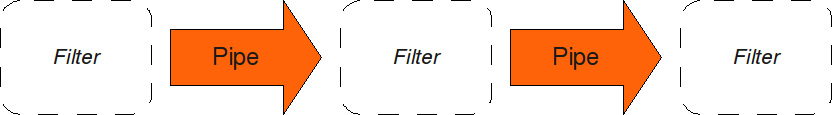
\includegraphics[scale=0.7]{pics/pipesFilter21.png}
	\caption[Pipes and Filter 2]{
	\textbf{Das Pipes and Filters Pattern.}
	Ein statisches Gerüst, dazu dynamische Filter, die in Form von Plugins geladen
	werden \todo{ein bisschen genauer, schöner, detailreicher?}}
	\end{center}
	\label{fig:pipesFilter21}
\end{figure}

Die Pipeline teilt sich so in zwei Teilkomponenten:
Die \enquote{dynamischen Steps} und das \enquote{statisches Ausfürhungsgerüst}.